\section{VPS+asteriskでオレオレコールセンター}
\subsection{はじめに}

\begin{screen}
\begin{center}
突然ですが、きちんと起きることができますかー?
\end{center}
\end{screen}

はじめまして。@tboffice\footnote{https://twitter.com/tboffice}と申します。普段はモバイル系のwebサービスのインフラエンジニアぽいことをしています。よく書く言語はbashスクリプトです\footnote{grepたんsedたんawkたんprpr}。今回は、オレオレコールセンターを構築する話を書きます。

冒頭の質問に戻ります。あなたは、朝、ちゃんと起きていますか?言い訳してるんじゃないですか?早く起きるのは無理だって、諦めているんじゃないんですか?\footnote{駄目だ駄目だ!あきらめちゃだめだ!できる!できる!絶対にできるんだから!}そんなあなたに、最適なソリューションをお届けします。電話を自動でかけてもらう、モーニングコールサービスを作ります。

モーニングコールのサービスについてはいくつか種類があります。たとえば、人間が電話をかけてくれるサービス\footnote{モーニングコールどっとコム(http://www.morning-call.com/)}や、電話をとると音声を流すサービス\footnote{モーニングコール娘(http://hisui.on.arena.ne.jp/morning/pc/)や時報ちゃん(http://www.jihouchan.com/)}があげられます。ここでは、幸いなことにインフラエンジニアは電話が鳴るといつでも飛び起きるという習性があるので、これを利用します。

\subsubsection{手段}
モーニングコールをかけてもらうためには、どこかから電話をかけなければいけません。そもそも、電話とは何でしょうか。それだけで同人誌1冊できあがってしまうので省略します\footnote{知識が乏しいので説明回避してるだけ}。我々が電話を使うためには、固定電話回線を引くか、携帯電話か、IP電話かという選択肢があります。今回の目的を達成するには、ある程度自由が効く\footnote{人間が介さず、電話の発信・受信についてプログラマブルであるという意味}IP電話を使います。IP電話といっても、ざっくりとハードウエアとソフトウエアに分かれていて、ハードウエアの場合はYAMAHAのルータや、SOHO・中小企業向けのハードウエアを使うという選択肢があります。しかし、個人で使うには敷居が高いので、ハードウエアがごにょごにょしている部分をソフトウエアで実現しているasteriskを使います。asterisk単体だと内線システムを作ることができます。今回の目的である電話に発信や着信をするには、電話回線に取り次いでくれるプロバイダ\footnote{そのようなプロバイダをITSP(Internet Telephony Service Provider)という}への契約が必要になります。

電話回線に取り次いでくれるプロバイダといば、NTTのフレッツのひかり電話や、ASAHI-NETのIP電話cなどです。もしご自宅でそれらのサービスと契約していれば、それをそのままつかいます\footnote{事例はネットに転がっているので参照してください}。今回はそれらのサービスを使わず、プロバイダに依存しないアジルネットワークスのクラウドPBXを使います。asteriskは、筆者が契約していたVPSにインストールします。

ここまでをまとめると、VPSにasteriskをインストールし、アジルクラウドPBXと契約してモーニングコールを行うオレオレコールセンターを構築します。簡単に今回の流れを図にまとめるとこうなります。

\begin{figure}[htbp]
 \begin{center}
  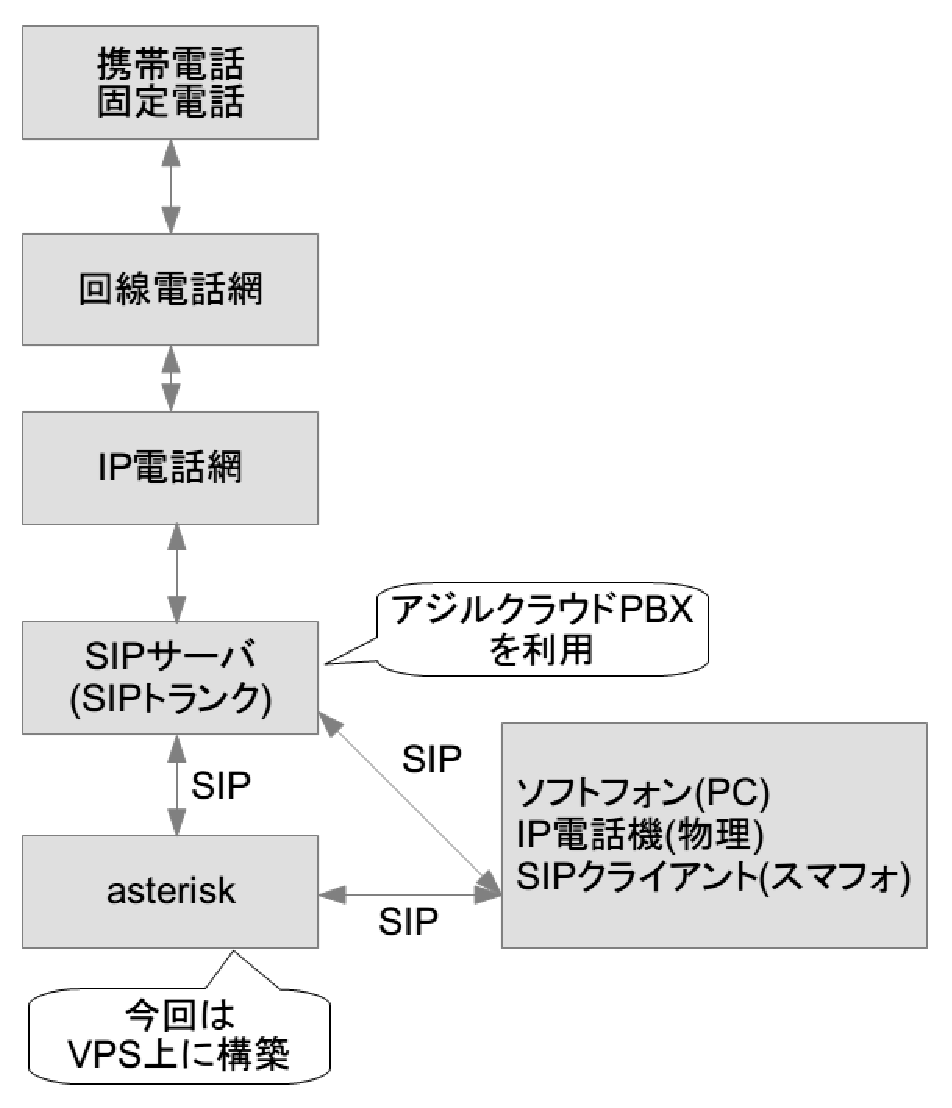
\includegraphics[width=70mm]{tboffice-asterisk/img/gaiyou.eps}
 \end{center}
 \caption{構築するシステム図}
 \label{fig:gaiyou}
\end{figure}

\subsubsection{asteriskとは}
GPL2ライセンスのIP-PBXのソフトウエアです。SIPをしゃべることができるので、電話回線に取り次いでくれるプロバイダが提供しているSIPとおしゃべりして、携帯電話や固定電話などへ着信や発信ができます。ただし、実際に発信着信するためにはソフトフォンやSIP対応の電話機などが必要です\footnote{もちろん常時インターネットに接続されていることが必要です}。ダウンロードや設定ファイルの書き方は、asterisk の公式サイト www.asterisk.org を参照してください。

\begin{figure}[htbp]
 \begin{center}
  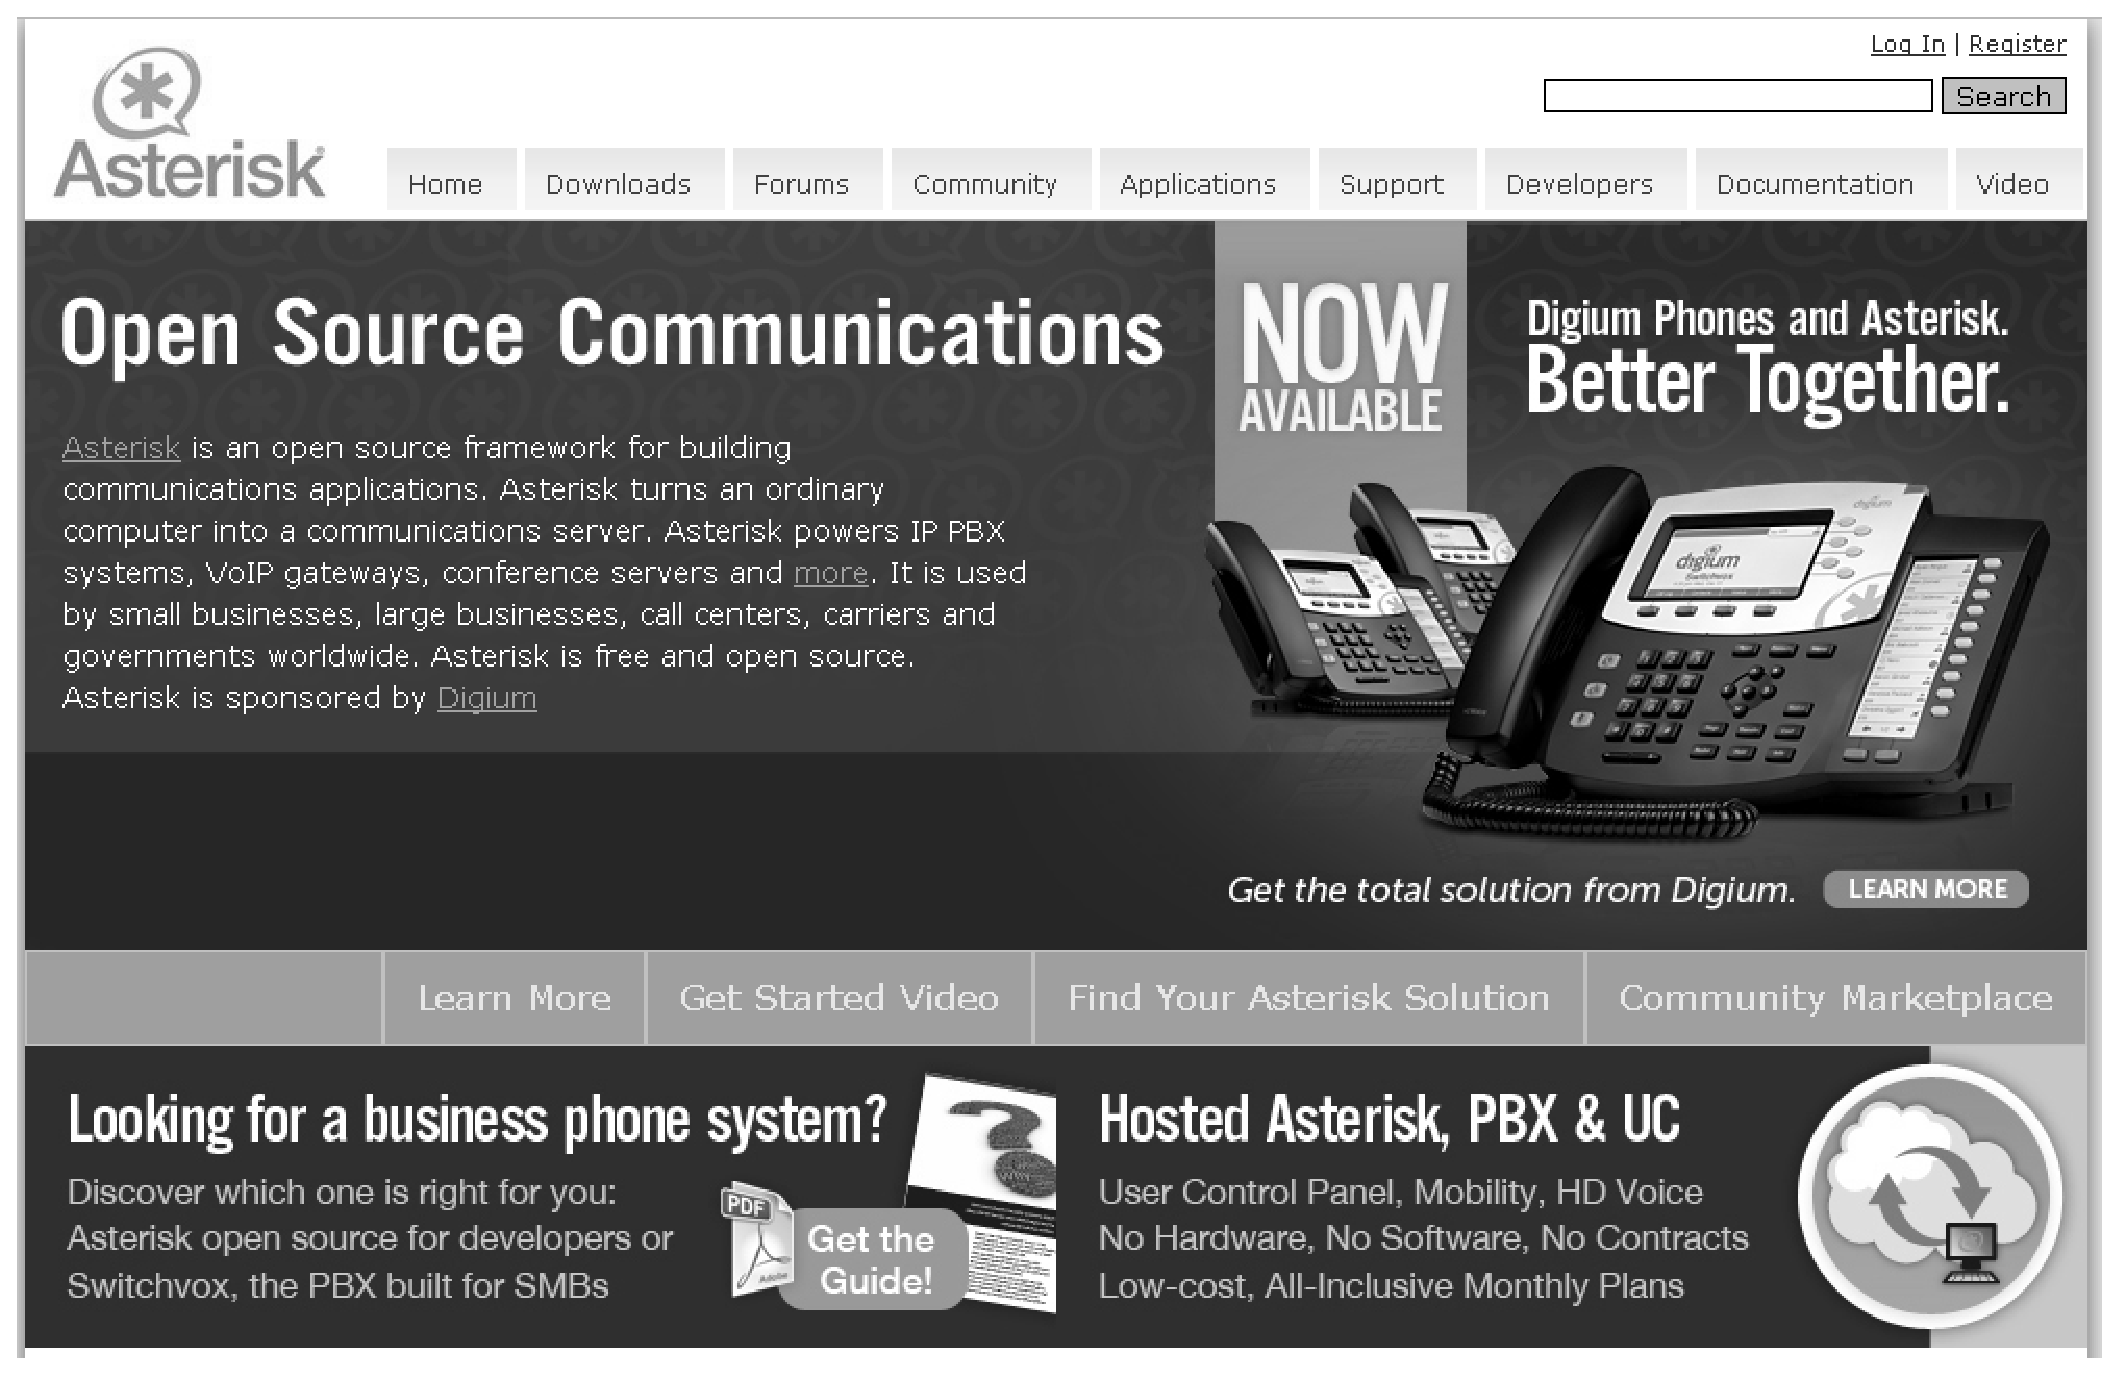
\includegraphics[width=100mm]{tboffice-asterisk/img/asterisk-site.eps}
 \end{center}
 \caption{www.asterisk.org}
 \label{fig:asterisk-site}
\end{figure}


\subsubsection{\textbf{!注意!}}
ここで解説する方法は、電話番号に対して電話をかけることができるので、電話番号の間違いには十分注意してください。冗談抜きのいたずら電話は絶対にするなよ!おっちゃんとの約束だぞ!!

\subsubsection{アジルクラウドPBXと契約}
アジルクラウドPBXに申し込みましょう。「SIPトランク」と「電話番号」を契約します。SIPトランクを契約すると、SIPサーバのサーバ名が払い出されます。初期費用は1800円、月額1800円(月途中は日割り)です。

電話番号は、東京03, 大阪06, 横浜045や、050などの番号を初期費用200円、月額200円/番号で取得することが出来ます。住んでもいないところの市外局番がとれるのは、なんともクラウドらしいですね。ちなみに0120もとれますが、お値段張ります。0120に限らず、取得できる電話番号はある程度プールを持っているらしく、検索することが出来ます。が、なかなかよい番号はないです。申し込んでから使えるようになるまで2-3日くらいかかります。

\subsubsection{VPSと契約}
筆者は、たまたまKDDIウェブコミュニケーションズのCloudCoreVPS\footnote{http://www.cloudcore.jp/vps/}の基本スペックで契約していたのでそれを使います。asteriskをインストールできる環境さえあれば、自宅サーバでもよいです\footnote{もし自宅サーバで、ローカルIP配下にasteriskサーバがある場合は「NAT越え」というハードルを越えてください。今回、グローバルipが直接ついているサーバを使っているので、説明は省きます}。VPSのスペックは、メモリ2G、CPUは1core 2.2G \footnote{AMD Phenom(tm) 9550 Quad-Core Processor /proc/cpuinfoより}、OSはCentOS 5.8 64bit版です。

\subsection{環境構築}
\subsubsection{asteriskをインストールする}

まず、VPSの環境は、ほぼデフォルトの状態だったので、足りないパッケージをインストールします。

\begin{lstlisting}[language=bash]
# yum install gcc gcc-c++ make libxml2-devel libtermcap-devel
\end{lstlisting}

次に、アジルフォンが推奨しているasteriskのバージョンをインストールします\footnote{本当は1行ですが、はみ出すので改行しています}。

\begin{lstlisting}[language=bash]
$ wget http://downloads.asterisk.org/pub/telephony/
asterisk/old-releases/asterisk-1.6.2.9.tar.gz
\end{lstlisting}

tar.gzがダウンロードできたら、適当なディレクトリに解答してコンパイルします\footnote{のーみそこねk}。prefix は好みで。ディレクトリ構成が独特ですがそのうち慣れます\footnote{make menuconfigまたはcmennuconfigあたりで、asteriskで使うモジュールの選択ができます。うまく使えば、バイナリサイズの圧縮になります。ただしモジュールがものすごく多いので気をつけてください}。

\begin{lstlisting}[language=bash]
$ ./configure --prefix=/usr/local/asterisk
$ make
# make install ; make samples ; make config
\end{lstlisting}

prefixに合わせて起動スクリプトを修正します。

\begin{lstlisting}[language=bash]
$ vi /etc/init.d/asterisk
\end{lstlisting}

AST\_CONFIGとAST\_SBINを下記に書き換え。

\begin{lstlisting}
AST_CONFIG=/usr/local/asterisk/etc/asterisk
AST_SBIN=/usr/local/asterisk/sbin
\end{lstlisting}

\subsubsection{asteriskをasteriskユーザで起動したいとき}
デフォルトではasteriskはroot権限で動作します。asteriskユーザで起動したいときは、asteriskユーザを作って /etc/init.d/asterisk の下記を設定します。

\begin{lstlisting}[language=bash]
AST_USER="asterisk"
AST_GROUP="asterisk"
\end{lstlisting}

あわせて、インストール後に、asterisk.conf の astctlowner と astctrlgroup を asterisk にしておくと吉。後述の cli で使うときにつかうソケットファイルのowner, groupとなります。

\subsubsection{asteriskを設定する}
重要なのは下記の2ファイルです。
\begin{itemize}
\item sip.conf
\item extensions.conf
\end{itemize}
これらのファイルは、/usr/local/asterisk/etc/asteriskにあります。設定ファイルの基本的な書き方はこのようになります。

\begin{lstlisting}[language=bash]
[samplesection]
key=value
object=>name
; comment 
\end{lstlisting}

key=value や object=\textgreater name は、[samplesection] のグループの中で有効という意味です。「;」はコメント行です。

ここではアジルクラウドPBXのasteriskの設定ファイルの設定方法はアナウンスされているのでそれを参照しました\footnote{http://www.agile.ne.jp/pdf/asterisk.pdf}。重要なのは、sip.confのcontextの値は、extension.confのディレクティブに対応する、ということです。これは重要です\footnote{大事なことなので(ry}。

/usr/local/asterisk/etc/asterisk/sip.conf ファイルを見ていきましょう。ITSPに接続するためのアカウント情報などを書きます。

\begin{lstlisting}[language=bash,basicstyle=\scriptsize]

[general]
allowguest=no
maxexpirey=3600
defaultexpirey=3600
port=5060
bindaddr=0.0.0.0
srvlookup=yes
disallow=all
allow=ulaw
language=jp

register => 000020XXXX: passwd@marika
;register => 58XXXXXX: passwd@chiaki

[marika]
type=friend
username=0000XXXXXX
secret=bentenmaru
context=autocall
canreinvite=no
host=voip30XX.agile.ne.jp
insecure=port,invite
disallow=all
allow=ulaw
fromuser=03XXXXXXXX

[chiaki]
type=friend
username=58XXXXXX
secret=passwd
context=inbound
canreinvite=no
host=smart.0038.net
insecure=port,invite
disallow=all
allow=ulaw

[200]
type=friend
username=200
secret=fuga
host=dynamic
context=outbound-1

\end{lstlisting}

次に、 /usr/local/asterisk/etc/asterisk/extensions.conf をみてみましょう。かかってきた電話に対してどのような動作をするのかを記述しています。

\begin{lstlisting}[language=bash,basicstyle=\scriptsize]
[general] 
writeprotect=no 
priorityjumping=yes 

[globals] 
AGILE_NUMBER=03XXXXXXXX
FUSION_NUMBER=58XXXXXX

[default] 
exten => 999,1,Set(CALLERID(num)=${AGILE_NUMBER}) 
exten => 999,n,Set(CALLERID(name)=${AGILE_NUMBER})
exten => 999,n,MP3Player(/tmp/Hacking_to_the_Gate.mp3) 
exten => 999,n,Hangup 

[inbound] 
exten => ${AGILE_NUMBER},1,Answer 
exten => ${AGILE_NUMBER},n,Dial(SIP/200,10,t) 
exten => ${AGILE_NUMBER},n,MP3Player(/tmp/Hacking_to_the_Gate.mp3) 
exten => ${AGILE_NUMBER},n,Busy(3)
exten => ${AGILE_NUMBER},n,Hangup 

exten => ${FUSION_NUMBER},1,Answer
exten => ${FUSION_NUMBER},n,Dial(SIP/200,10,t)
exten => ${FUSION_NUMBER},n,MP3Player(/tmp/Hacking_to_the_Gate.mp3)
exten => ${FUSION_NUMBER},n,Busy(3) 
exten => ${FUSION_NUMBER},n,Hangup

[autocall]
exten => 9999,1,Set(CALLERID(num)=${AGILE_NUMBER})
exten => 9999,n,Set(CALLERID(name)=${AGILE_NUMBER})
exten => 9999,n, MP3Player(/tmp/Hacking_to_the_Gate.mp3)
exten => 9999,n,Hangup

\end{lstlisting}

だいたいこんな感じです\footnote{モーパイみながら設定したからこうなっているのは内緒。fusionという記述が見えますがあとで補足します}。いつみてもキモイ記述方法ですね\footnote{遠い目をしながら}。電話をかけたら、MP3ファイルを再生するようにしています。あらかじめ、``Hacking\_to\_the\_Gate.mp3''というMP3のファイル\footnote{ファイルパスが長かったので/tmpにしていますが、もともとは/usr/local/asterisk/var/lib/asterisk/sounds/Hacking\_to\_the\_Gate.mp3に配置しています}を用意しておきます\footnote{選曲の理由はシュタゲ好きの人がいたので。ここだけの話、pediarouteの人らしいですよ}。mp3を再生するにはmpg123が必要なので、サーバにインストールされているか調べておきましょう。用意できれば、asteriskを起動しみます。

まず、asteriskを起動スクリプトでデーモンとして起動する前に、asteriskをCLIモード(コマンドで起動モード)で起動して様子を見ましょう\footnote{vはvorboseです。-vvvするほど、ログがうるさくなります。vは10個まで付けることが出来ます。同じく-d(debug)もあり-vと同じ効果をもたらすでしょう}。

\begin{lstlisting}[language=bash]
# /usr/local/asterisk/sbin/asterisk -cv
\end{lstlisting}

赤で表示されるErrorが出ていなければよいです。接続先のSIPサーバと疎通し、パスワードも通っていて、コマンドを打って下記のように表示されれば、接続が出来ている状態です。

\begin{lstlisting}[language=bash]
hostname*CLI> sip show registry 
Host dnsmgr Username Refresh State Reg.Time 
marika:5060 N 000020XXXX 585 Registered Tue, 19 Jun 2012 03:28:45
1 SIP registrations. 
\end{lstlisting}

quitと入力してCLIモードを抜けます。ここでasteriskが終了します。ここまで確認できれば、asteriskをinitスクリプトで起動します\footnote{設定がまずい状態でasteriskをデーモンであげると起動の無限ループに突入するので注意}。

\begin{lstlisting}[language=bash]
# /etc/init.d/asterisk start
\end{lstlisting}

デーモンで起動したasteriskにCLIでつなぐときは下記のコマンドで可能です\footnote{困ったらTabを押せばなんとかなる}。さっきはcオプションを指定しましたが、今度はrオプションを使います。

\begin{lstlisting}[language=bash]
$ /usr/local/asterisk/sbin/asterisk -rv
\end{lstlisting}

さて、asteriskも起動したことなので、電話をかければmp3が再生されるはずです。あとはソフトフォン\footnote{筆者はなんとなくZoiperを使っています。ソフトフォンもいくつか種類があるので比べてみると良いです}でregiSterして電話番号を入力すると電話かかることを確認してください。横道にそれるのでこれ以上は説明しません。ヒントは、extensions.confの[200]ディレクティブです。

\subsubsection{モーニングコール}
電話をかけるファイルを用意します。

\begin{lstlisting}[language=bash]
# cat etc/autocall.dial 
Channel: SIP/080XXXXXXXX@marika
MaxRetries: 0
RetryTime: 15
WaitTime: 15
Context: autocall
Extension: 9999
\end{lstlisting}

電話をかけるファイルを実行するスクリプト

\begin{lstlisting}[language=bash]
# cat bin/autocall.sh 
#!/bin/bash
cp ~/etc/autocall.dial /usr/local/asterisk/var/spool/asterisk/outgoing/
# chmod +x bin/autocall.sh  #実行権限をつけるだけ
\end{lstlisting}
スクリプトを実行して、電話がかかってくることを確認しましょう。かかってこなかったら、設定に失敗しているか、だれか知らない人にかかっている可能性があります。
次に、crontabに登録します。
\begin{lstlisting}[language=bash]
# crontab -l 
0 7 * * * /root/bin/autocall.sh
\end{lstlisting}

もう一つ気をつけることは、/usr/local/asterisk/var/spool/asterisk/outgoing/に放り込まれたautocall.dialのファイルは、起動中のasteriskから読め、且つ、ファイルが消せる状態でないといけません。

\subsection{FUSION IP-Phone SMARTがやってきた}
話題はがらっと変わります。IP電話にも新しい風が入って参りました。フュージョンコミュニケーションズのFUSION IP-Phone SMARTというサービスが2012/5/15にベータ版でリリースされました。このサービスは、図のSIPサーバ(SIPトランク)にあたります。つまり、asteriskからregistered\footnote{SIPで接続ができるという意味。cliのコマンドでshow sip registry と打つとregisteredと出てくることから筆者はそう呼んでいます}できます。また基本料金が不要で、通話料のみで電話をかけることができます。そして、IP-Phone SMART同士ならタダ…アジルフォンを使う理由が薄まってしまいました。

今回の記事で、sip.conf, extensions.confに[chiaki]というディレクティブがありますが、実はそれがFUSION IP-Phone SMART用の設定です。設定はすでに書いてあるので、sip.confの下記の設定を有効にして\footnote{;をはずすだけ}asteriskを再起動\footnote{再起動がいやや、という方はCLIでconfig reload /usr/local/asterisk/etc/asterisk/sip.confしてもおk}すると、FUSION IP-Phone SMARTとregistered状態となります。

\begin{lstlisting}
register => 58XXXXXX: passwd@chiaki
\end{lstlisting}

アジルクラウドPBXを使うメリットは、IP電話と分かられない電話番号\footnote{050 で始まらない番号}が取得できるくらいですかね。アジルフォン側で設定次第で会話の録音をやってくれますが、asteriskでextension書けば、通話の録音は出来るはず\footnote{未検証}。


私自身は、iphoneのSIPクライアントアプリであるmedia5-Fone for iPhone\footnote{http://www.media5corp.com/en/softphones/media5-fone-iphone/}で直接SIPサーバとregisteredして使っています。アジルフォンとIP電話同士で音質がどうなるのか検証用です。着信をするなら、アプリでSIPクライアントアプリを常時起動しておかねばならず、電池を食います。
\begin{figure}[htbp]
 \begin{center}
  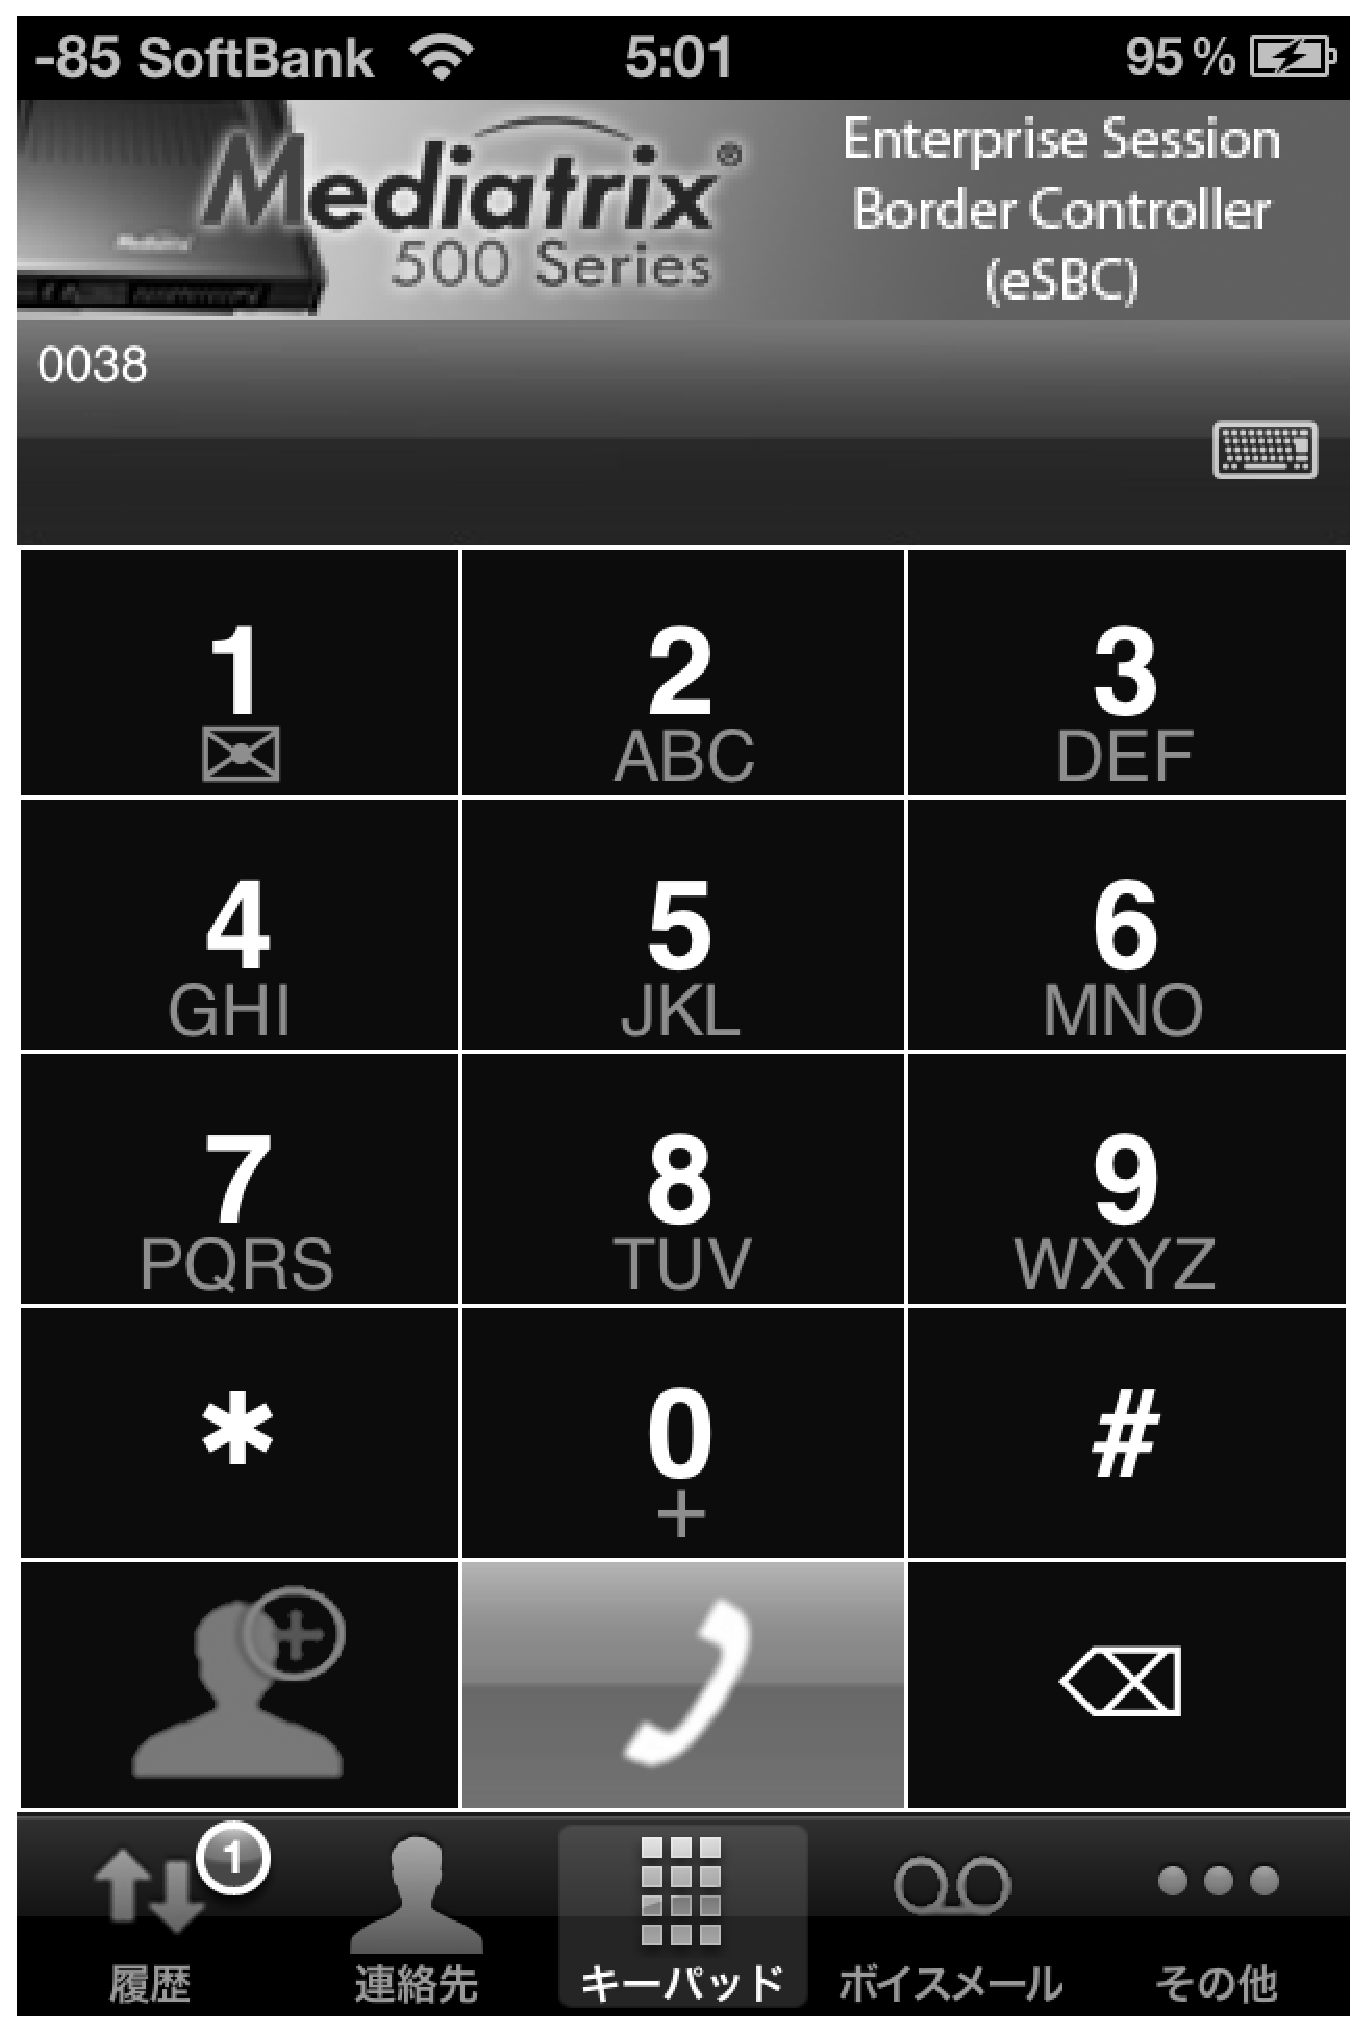
\includegraphics[width=50mm]{tboffice-asterisk/img/media5.eps}
 \end{center}
 \caption{media5-Fone for iPhoneの起動中画面}
 \label{fig:media5}
\end{figure}

\subsection{まとめ}
asteriskは企業の内線電話を低価格で実現できる用途で使うのが一般的\footnote{http://voip-info.jp/index.php/導入事例}です。asteriskの記事を初心者向けに書くなら、「ソフトフォン \textless = \textgreater asterisk \textless = \textgreater ソフトフォン」の設定をやって「オレオレSkypeサーバ」などから始めるのが一般的だとは思います。asteriskを全く知らない人にしてみれば、この自動発信はかなり敷居が高いと思います。ITSPの契約や、SIPサーバの接続の方法、設定ファイル、outgoingファイルを理解しないといけません。さらに運用面では、セキュリティーにも注意しないといけません。SIPポートにアクセスしてきてアカウントを総当たりし、勝手に電話をかけられてしまう可能性があります\footnote{http://www.voip-info.jp/index.php/Asterisk\_SIP\_セキュリティ}。もちろん発信者がお金を払うので、ちまたで流行のクラウドPBX破産\footnote{きぃたことねぇよ}が起きるかもしれません。十分注意しましょう。

\subsubsection{実際に運用してみて}
携帯のアラームでも、人間の耳にとっては同じです\footnote{当たり前}。携帯の画面を見ると、発信者の電話番号が書いてあります。それを見ることによって、比較的起きる確率は上がったように感じます\footnote{小学生のころ、小学生新聞なるものがありまして、相談コーナーというものがありました。「朝早く起きるには」という問いに対して、「強い意志が必要」と回答がありました。今見ても至言だと思います。修造も言っています。あきらめちゃだめだ!できる!できる!絶対にできるんだから!}。逆に、携帯のアラームで画面に着信しているように見せかける着メロがあれば…いやー売れないだろう\footnote{そもそもキャリアに怒られそう}。

\subsection{次回}
iPhoneでSIPアプリ立ち上げておくと思ったより電池が減ります。appleのPUSH通知でアプリ起動できるらしいという噂話を聞いたので挑戦してみたいところ。あるいは基本に戻ってオレオレSkypeなど要望があれば書くかもしれません。はたまた全く別のことを書くかもしれません。

\subsection{参考文献}
\begin{itemize}
\item Asterisk- The Open Source Telephony Projects | Asterisk - http://www.asterisk.org/
\item 『Asterisk 運用・開発ガイド』 オーム社
\item VOIP-Info.jp Wiki - http://www.voip-info.jp
\item asteriskでモーニングコール - http://enjoy.potix.jp/diary/asteriskでモーニングコール
\item agile networks TOP | アジルモバイルセントレックス、アジルクラウドPBX | アジルネットワークス株式会社 - http://www.agile.ne.jp/
\end{itemize}
